\documentclass[11pt]{article}
\usepackage{amsmath,amssymb,amsthm,tikz}

\DeclareMathOperator*{\E}{\mathbb{E}}
\let\Pr\relax
\DeclareMathOperator*{\Pr}{\mathbb{P}}

\newcommand{\eps}{\varepsilon}
\newcommand{\inprod}[1]{\left\langle #1 \right\rangle}
\newcommand{\R}{\mathbb{R}}

\newcommand{\handout}[5]{
  \noindent
  \begin{center}
  \framebox{
    \vbox{
      \hbox to 5.78in { {\bf CS 224: Advanced Algorithms } \hfill #2 }
      \vspace{4mm}
      \hbox to 5.78in { {\Large \hfill #5  \hfill} }
      \vspace{2mm}
      \hbox to 5.78in { {\em #3 \hfill #4} }
    }
  }
  \end{center}
  \vspace*{4mm}
}

\newcommand{\lecture}[4]{\handout{#1}{#2}{#3}{Scribe: #4}{Lecture #1}}

\newtheorem{theorem}{Theorem}
\newtheorem{corollary}[theorem]{Corollary}
\newtheorem{lemma}[theorem]{Lemma}
\newtheorem{observation}[theorem]{Observation}
\newtheorem{proposition}[theorem]{Proposition}
\newtheorem{definition}[theorem]{Definition}
\newtheorem{claim}[theorem]{Claim}
\newtheorem{fact}[theorem]{Fact}
\newtheorem{assumption}[theorem]{Assumption}

% 1-inch margins, from fullpage.sty by H.Partl, Version 2, Dec. 15, 1988.
\topmargin 0pt
\advance \topmargin by -\headheight
\advance \topmargin by -\headsep
\textheight 8.9in
\oddsidemargin 0pt
\evensidemargin \oddsidemargin
\marginparwidth 0.5in
\textwidth 6.5in

\parindent 0in
\parskip 1.5ex

\begin{document}

\lecture{24 --- April 14, 2017}{Spring 2017}{Prof.\ Jelani Nelson}{Evan Yao}

\section{Overview}

In the last lecture we looked at the multiplicative weights (MW) algorithm as well as a variation of the $n$ experts problem where we are asked to give a probability distribution $p^{(t)}$ at each iteration. We started using MW to give a solution to LP's in general. 

In this lecture we will finish the analysis of LP's with the multiplicative weights algorithm and then start talking about network flows. 

\section{Recap}

Recall the $\gamma$ bounded oracle from last lecture: 

\begin{definition} 
In a {\em $\gamma$-Bounded Oracle}, we are given $p$, a probability distribution over the rows of $A$. If $$\{x \in P,~ p^T Ax  \geq p^T b\}$$ is feasible, then it returns such a feasible $x$ with the following property: 
$$ \forall i \left| \langle A_i, x\rangle - b_i \right| \leq \gamma$$ 
\end{definition}

Note that this is an easier feasibility problem than satisfying $\{ x \in P, Ax \geq b\}$. This oracle says that if the former is feasible, then we can find a $x$ satisfying the former that \textbf{almost} satisfies the latter (if $\gamma$ is small). Each dimension can be off by a factor of $\gamma$. 


In the last lecture, we proved the following bound for the variation of the experts problem where we are asked to give a probability vector $p^{(t)}$ at each time step. For all $\eta \in (0, \frac{1}{2}]$, this algorithm achieves the following bound:

\begin{align*}
    \sum_{t = 1}^T \langle m^{(t)} ,p^{(t)} \rangle &\leq \min_{1\leq i\leq n}  \left(\sum_{i}m_i^{(t)} + \eta \sum_{t=1}^T |m_i^{(t)}| \right) + \frac{\ln n}{\eta}\\  &\leq \min_{i} \sum_{t=1}^T m_it + \eta T + \frac{\ln n}{ \eta}
\end{align*}  

The second inequality follows since we assume that $m_i^{(t)}\in[-1,1]$ for all $i,t$. Today, we will combine this algorithm and this bound with a $\gamma$ bounded oracle in order to solve LP's using MW.

\section{Using Oracle together with MW} 
Recall the setup for the problem. There is a convex region $P$ as well as $A\in\R^{m\times n}$ and $b\in\R^n$. We would like to decide feasibility of $\{x\in P, Ax \ge b\}$. If this problem is feasible, we would like to find $x\in P$ satisfying $Ax\ge b - \epsilon\cdot J$, where $J$ is the all ones vector.

The MW-based algorithm runs as follows: 
\begin{itemize}
\item 
Initialize $p^{(1)}$ to be the uniform distribution over the $m$ rows of $A$ 
\item 
Each row of $A$ is an expert, so there are $m$ experts. 
\item Use $p^{(t)}$ to get $x^{(t)}$ from the oracle. Output ``infeasible'' if the oracle says infeasible. 

\item Once we get back this $x^{(t)}$, we define $m_i^{(t)} = \frac{1}{\gamma} \cdot \left( \langle A_{i}, x^{(t)} \rangle - b_i\right)$. We know that the absolute value of $m_i^{(t)}$ is less than 1 because of the gamma bounded oracle gives you an $x^{(t)}$ such that $ \left| \langle A_i, x^{(t)}\rangle - b_i \right| \leq \gamma$.

Notice that if a constraint $i$ is well-satisfied, $m_i^{(t)}$ will be close to 1, and if it is very unsatisfied, then $m_i^{(t)}$ will be close to $-1$.

\item Based on $m^{(t)}$ and $p^{(t)}$, we then obtain $p^{(t+1)}$ via the MW update rule from last lecture.

\end{itemize}

\begin{theorem} 
$\forall \epsilon \in (0,1)$, if we have a $\gamma$ bounded oracle for $\gamma \geq \epsilon /2$, then we can find $x$ such that $x \in P$, $Ax \geq b - \epsilon \cdot J$ in $O(\frac{\gamma^2 \ln m}{\epsilon^2})$ iterations (i.e. days) of multiplicative weights. 
\end{theorem}

Note if $\gamma < \epsilon/2$, we can just redefine $\gamma$ to be $\epsilon/2$.

\begin{proof} 

For any time period $t$, we have: 
\begin{align*}
    \langle m^{(t)}, p^{(t)} \rangle &=  (p^{(t)})^T m^{(t)} \\ 
    &= \frac{1}{\gamma} (p^{(t)})^T \left( Ax^{(t)} - b \right) \\
    &= \frac{1}{\gamma} \left( (p^{(t)})^T Ax^{(t)} -(p^{(t)})^T b \right) \\
    &\geq 0 .
\end{align*}
Note that $(p^{(t)})^T$ refers to the \textit{transpose} of the vector $p^{(t)}$. To get the last step, we used the fact that $x^{(t)}$ was returned by the oracle and thus satisfies $\{x \in P, p^T A  \geq p^T b\}$. Once we have the above inequality, we sum over all $t$ so that for all (constraints) $i$: 
\begin{align*}
    0 &\leq \sum_{i=1}^{T} \langle m^{(t)}, p^{(t)} \rangle \\ 
    &\leq \sum_{t=1}^T m_i^{(t)} + \eta T + \frac{\ln m}{\eta} \\ 
    &\leq \frac{1}{\gamma}\sum_{t=1}^T \left( \langle A_i, x^t \rangle - b_i \right) + \eta T + \frac{\ln n}{\eta}\\
    \intertext{Now, let $x = \frac{1}{T} \sum_{t=1}^T x^{(t)}$. By the linearity of the inner product, we have:}
    0&\leq \frac{T}{\gamma} \cdot \langle A_i, x \rangle - \frac{T}{\gamma} \cdot b_i + \eta T + \frac{\ln n}{\eta} \\
    \intertext{Dividing through by $\frac{T}{\gamma}$ gives us:}
    0 &\leq \langle A_i, x\rangle - b_i + \gamma \eta + \frac{\ln n \cdot \gamma}{\eta \cdot T}
\end{align*}
Now, it is just a matter of choosing $\eta$ and $T$ so that $\gamma \nu + \frac{\ln n \cdot \gamma}{\eta \cdot T} \leq \epsilon$. Choose $\eta \leq \frac{\epsilon}{2\gamma}$ and then choose $T \geq \frac{2\gamma \ln m}{\eta}$. This will make both terms less than $\frac{\epsilon}{2}$. 

This implies: 
$$ \langle A_i, x \rangle \geq b_i - \epsilon$$ 
for each row $i$ of $A$. Hence, we know that
$$ Ax \geq b - \epsilon \cdot J$$ 

Therefore, it suffices to run multiplicative weights for $T \geq \frac{2 \gamma \ln m}{\eta \epsilon} \geq \frac{4 \gamma^2 \ln m}{\epsilon^2}$ iterations. 
\end{proof}

\section{Flows}

\subsection{Setup}
\begin{itemize}
\item We are given a directed graph $G = (V,E)$ with a source $s \in V$ and sink $t \in V$. 
\item Each edge $e$ of the graph has a capacity $u_e \in \{1,2, \ldots, U\}$. 
\item Our goal in max flow is "route" as much flow as possible from $s$ to $t$. 
\end{itemize}
\textbf{Intuition: }The source $s$ is an infinite source of water while the sink $t$ can accept an infinite pool of water. The capacity of each pipe is the amount of water that can go through it per unit of time. We are trying to find the maximum amount of water that can be transported, per unit of time, from $s$ to $t$. 

\textbf{Example: } In the graph below, it is possible to send 2 units of flow from $s$ to $t$. However, the greedy algorithm of choosing paths from $s$ to $t$ and filling them completely does not work. If we choose the path $s \to a \to d \to t$ and put 1 unit of flow on that edge, then there is no way to find another path from $s$ to $t$ to send the other unit of flow. 
\begin{center}
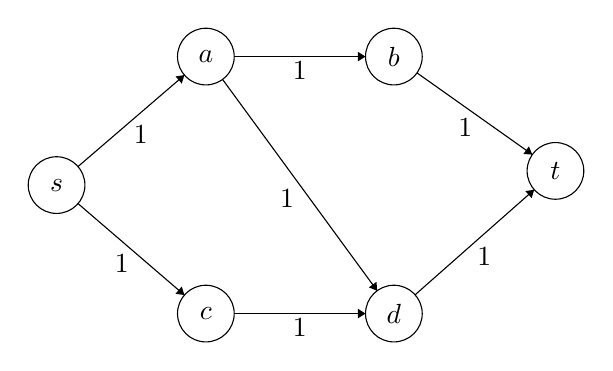
\begin{tikzpicture}[scale=0.12]
\tikzstyle{every node}+=[inner sep=0pt]
\draw [black] (30.9,-18.2) circle (3);
\draw (30.9,-18.2) node {$a$};
\draw [black] (50.8,-18.2) circle (3);
\draw (50.8,-18.2) node {$b$};
\draw [black] (15.1,-31.8) circle (3);
\draw (15.1,-31.8) node {$s$};
\draw [black] (30.9,-45.4) circle (3);
\draw (30.9,-45.4) node {$c$};
\draw [black] (50.8,-45.4) circle (3);
\draw (50.8,-45.4) node {$d$};
\draw [black] (67.9,-30.3) circle (3);
\draw (67.9,-30.3) node {$t$};
\draw [black] (17.37,-29.84) -- (28.63,-20.16);
\fill [black] (28.63,-20.16) -- (27.69,-20.3) -- (28.35,-21.06);
\draw (24.01,-25.49) node [below] {$1$};
\draw [black] (33.9,-18.2) -- (47.8,-18.2);
\fill [black] (47.8,-18.2) -- (47,-17.7) -- (47,-18.7);
\draw (40.85,-18.7) node [below] {$1$};
\draw [black] (53.25,-19.93) -- (65.45,-28.57);
\fill [black] (65.45,-28.57) -- (65.09,-27.7) -- (64.51,-28.51);
\draw (58.35,-24.75) node [below] {$1$};
\draw [black] (53.05,-43.41) -- (65.65,-32.29);
\fill [black] (65.65,-32.29) -- (64.72,-32.44) -- (65.38,-33.19);
\draw (60.36,-38.34) node [below] {$1$};
\draw [black] (33.9,-45.4) -- (47.8,-45.4);
\fill [black] (47.8,-45.4) -- (47,-44.9) -- (47,-45.9);
\draw (40.85,-45.9) node [below] {$1$};
\draw [black] (17.37,-33.76) -- (28.63,-43.44);
\fill [black] (28.63,-43.44) -- (28.35,-42.54) -- (27.69,-43.3);
\draw (21.99,-39.09) node [below] {$1$};
\draw [black] (32.67,-20.62) -- (49.03,-42.98);
\fill [black] (49.03,-42.98) -- (48.96,-42.04) -- (48.15,-42.63);
\draw (40.27,-33.19) node [left] {$1$};
\end{tikzpicture}
\end{center}


\begin{definition} 
A flow $f$ is a vector in $\mathbb{R}^m$ such that the following properties hold:
\begin{itemize}
\item Nonegativitiy: $$f_i \geq 0$$ for each coordinate of $f$.
The flow through an edge cannot be negative. 
\item Conservation of Flow: $\forall u \in V \setminus \{s,t\}$

$$\sum_{e = (u, \cdot)} f_{e} = \sum_{e = (\cdot, u)} f_e$$

The sum of the water going in and coming out of a vertex (not the source or sink) must be equal. 

It follows from conservation of flow that the amount of flow exiting the source is the same as the amount entering the sink. 

\item Capacity: 
$\forall e$ $$f_e \leq u_e$$
The flow through an edge must obey that edge's capacity constraint. 
\end{itemize}

The objective is to maximize the flow coming out of $s$ or equivalently the flow flowing into $t$:

$$ \max \sum_{e = (s, \cdot)} f_e = \max \sum_{e = (\cdot, t)} f_e $$
\end{definition}

\subsection{Current Literature}
In this section, we will look at some of the existing algorithms for solving max flow. Sometimes, we will use $\tilde{O}$ instead of $O$ to hide polylogarithmic factors. We will also use the standard notation of $m$ being the number of edges and $n$ being the number of vertices. Without loss of generality, we assume that $m \geq n-1$ (in a pre-processing step we can throw away all vertices which are not reachable from $s$).

\textbf{Interior Point Methods: }

Using interior point methods, we can solve the LP for max flow in $\tilde{O}(\sqrt{m'}L)$ iterations of interior point, where $m'$ is the number of constraints in the max flow LP. Each iteration is $O(1)$ Newton steps, where we have 
$$ x^{k+1} \leftarrow x^{k} - \left( \nabla^2 f(x_k) \right)^{-1} \nabla f(x_k)$$ 

Another way of thinking about this is $$ \nabla^2 f(x_k) \left( x_{k} - x_{k+1}\right) = \nabla f(x_k) $$

and so finding $x_{k+1}$ can be done by solving a system of linear equations. 

Let $A$ be the constraint matrix in the LP formulation of max flow. What are the dimensions of $A$? The max flow LP has $m$ variables and $m' = \Theta(m+n)$ constraints, one for edge's capacity and non-negativity and one for each vertex's conservation of flow. But we assumed that $m \geq n-1$ and thus both dimensions of $A$ are $\Theta(m)$. We can solve a system of linear equations in the same time as matrix multiplication, which naively is $O(m^3)$. Therefore, we can solve this LP via the interior point method with run-time

$$\tilde{O}(\sqrt{m} m^3 \cdot L) = \tilde{O}(m^{7/2} \lg U)$$ 

Using our definiton of $L$ from the interor point method, it can be shown that $L = O(\lg U)$ for max flow.

Daitch and Spielman proved in \cite{Daitch} that the matrices $A$ we get from the max flow problem are special so that you can solve linear systems in $\tilde{O}(m)$ time. This means that max flow can be solved in time $\tilde{O}(m^{3/2} \lg U)$. 


Recall the objective function from the interior points method: $f_\lambda(x) = \lambda c^T x - \sum_{i=1} \ln (s(x_i))$. There's something interesting about optimizing this function, which is that if you take a linear problem and you repeat a constraint a million times, you've incremented $m$, but you really haven't fundamentally changed the problem at all. Lee and Sidford found an algorithm in \cite{Lee} such that the number of iterations of interior point it runs would not increase even if constraints were duplicates or near duplicates of each other. At a (very) high level, they did this by weighing each of the constraints in the barrier function depending on how important they were based on the polytope itself. This led to $\tilde{O}( m \sqrt{n} \lg U)$ max flow solution (and fast linear programming overall).

\textbf{Summary Table}

The table below summarizes the above as well as adds some other max flow algorithm landmarks: \begin{center}
\begin{tabular}{lll}
    Authors & Run-time & Remark  \\ \hline
    Daitch and Spielman \cite{Daitch} & $\tilde{O} (m^{3/2} \lg U)$ & $A$ is a special matrix in max flow \\ 
    Lee and Sidford \cite{Lee} & $\tilde{O}(m\sqrt{n} \lg U)$ & Interior-point based approach \\ 
    Madry \cite{Madry} & $\tilde{O}((mU)^{10/7})$ & Pseudopolynomial \\ 
    Goldberg and Rao \cite{Goldberg} & ${\scriptstyle O(m \cdot \min( \sqrt{m}, n^{2/3} ) \cdot \lg(n^2/m) \lg U)}$ & Weakly Polynomial \\
    Orlin \cite{Orlin} & $O(mn + m^{31/16} \lg^2 n)$ & Strongly Polynomial\\
    King, Rao, and Tarjan \cite{King} & $ O( mn \cdot \log_{m/ (n \log n)} n)$ & Min of \cite{Goldberg} and \cite{King} is $O(mn)$
    
\end{tabular}
\end{center}


\textbf{Minimum Congestion Flow}

In undirected graphs, Kelner et al.\ \cite{Kelner} and Sherman \cite{Sherman} showed that we can get running time $O(m^{1 + o(1)} / \epsilon^2)$ to find at least $(1-\epsilon)$ of the max flow. This was improved to $\tilde{O}(m/\epsilon^2)$ by Peng in \cite{Peng}. The idea for these algorithms is to use the idea that maximum flow is equivalent to minimum congestion flow. 

\begin{definition}
For the \textbf{Minimum Congestion Flow} problem, we want to send 1 unit of flow from $s$ to $t$. The cost of the flow is the maximum of $f_e/u_e$. We want to minimize this cost.
\end{definition}

These two problem are equivalent because we can find simply divide all the $f$'s by the value of the max flow. This will result in 1 unit of flow being transmitted. 

Define a matrix $B \in \mathbb{R}^{m \times n}$ such that the rows are indexed by the edges of $G$ and the columns are indexed by the vertices of $G$. For each row (edge), put 1, -1 at the $(u,v)$. 1 for $u$, $-1$ for $v$. 

We have a demand vector $\chi \in \mathbb{R}^{n}$. That vector describes each vertex's need to ship or absorb flow. Set $\chi$ to be $1$ in $s$ and $-1$ in $t$. $B^T f$ gives us an $n$ dimensional vector such that the $v$th entry is how much flow is being pushed out of $v$. If this quantity is negative, then this vertex is absorbing some flow, and if it is positive then some extra flow is spilling out of the vertex. Conservation is achieved when this entry is 0. 

Let $U$ be diagonal $m \times m$ matrix of all the edge capacities. Thus for the minimum congestion flow problem (equivalent to max flow), we wish to compute an $m$-dimensional vector $f^*$ such that $B^T f^* = \chi$ and $|| U^{-1} f^* ||_\infty$ is as small as possible. Here, we have a constrained optimization problem, so we can't use gradient descent. These papers try to remove those constraints and do gradient descent. You turn this into an unconstrained optimization problem by: Find some flow $f_0$ from $s$ to $t$ using DFS that satisfies the entire demand $\chi$. Look at $f^* - f_0$: this is a circulation, i.e.\ it routes the demand $\chi = 0$.

Then we wish to compute $$c^* = \text{argmin}_{B^T c = 0} || U^{-1} (f_0 + c) ||_\infty $$
Let $\alpha_0 = U^{-1} f_0$. To make this an unconstrained optimization problem, we project a vector $z\in\R^m$ onto ``circulation space'', which is just the linear subspace of all $z$ satisfying $B^{T} f = z$.  

$$z^* = \text{argmin}_{z \in \mathbb{R}^{m}} || \alpha_0 + U^{-1} P z||_\infty$$ where $P$ is a projection matrix. This is now an unconstrained optimization problem where $z$ is allowed to be anything in $\mathbb{R}^m$. Now one can use continuous optimization methods such as gradient descent, and the heart of these works is in designing a good projection matrix $P$ with certain nice properties that we won't get into here.

\section{Algorithms}

Today, we will look at the \textbf{Ford Fulkerson} algorithm \cite{Ford}. Its run-time is $O(m \cdot f^*)$ where $f^*$ is the value of the max flow. Ford Fulkerson works by initializing $f = 0$ and while there exists an $s-t$ path $p$ in the residual graph $G_f$, let $\lambda$ be the smallest capacity on edges in $p$ in the residual graph. Let $f'_e = \lambda $ for $e \in p$, $0$ otherwise. Update $f$ with $f + f'$. When there is no path left, return $f$. 

But what is the residual graph $G_f$? 

For notational convenience, let $f_{e} = -f_{r(e)}$ where $r(e)$ is the reverse edge of $e$. If $e\in E$, but $r(e)$ is not, then we'll pretend that $r(e) \in E$ with capacity $0$. The residual graph $G_f$ has the same vertex and edge sets as $G$, but with changed capacities. Its capacities $u'$ satisfy:

$$u'_e = u_e - f_e + f_{r(e)}$$

\textbf{Intuition}: When flow is being sent in one direction, we allow flow to travel in the opposite direction by ``pushing back'' flow.

We will state the following theorems, but will not prove them. You can refer to notes from CS 124 or CLRS for complete proofs. 

\begin{theorem} 
$f^*$ is a max flow iff there is no $s$-$t$ path in $G_f$ with positive minimum capacity.
\end{theorem}

\begin{theorem} 
The maximum $s$-$t$ flow is equal to the minimum $s-t$ cut. 
\end{theorem}
Recall that an $s$-$t$ cut is a partitioning of the vertices into 2 groups such that $s$ and $t$ are in different groups. The value of the cut is the sum of the capacities of all the edges leaving the $s$ side and towards $t$ side.

Next time, we will look at scaling algorithms for max $s$-$t$ flow, which will give us a running time like $O(m^2 \ln U)$ time. We will also look at blocking flow algorithms, which can combine with scaling to give a runtime of $O(mn \ln U)$. It is also possible to get $O(m \sqrt{n})$ in unit graphs, where every vertex besides $s$ and $t$ either have indegree 1 or outdegree 1, e.g.\ the kinds of graphs that arise when reducing maximum bipartite matching to maximum $s$-$t$ flow.

\bibliographystyle{alpha}

\begin{thebibliography}{42}

\bibitem{Daitch}
Samuel I. Daitch, Daniel A. Spielman.
\newblock Faster approximate lossy generalized flow via interior point algorithms. 
\newblock  {\em STOC 2008}: 451-460

\bibitem{Lee} 
Yin Tat Lee, Aaron Sidford.
\newblock
Path Finding Methods for Linear Programming: Solving Linear Programs in Õ(vrank) Iterations and Faster Algorithms for Maximum Flow. 
\newblock {\em FOCS 2014}: 424-433

\bibitem{Madry} 
Aleksander Madry. 
\newblock 
Computing Maximum Flow with Augmenting Electrical Flows. 
\newblock{\em FOCS 2016}: 593-602

\bibitem{Goldberg} 
Andrew V. Goldberg, Satish Rao:
\newblock 
Beyond the Flow Decomposition Barrier. 
\newblock
{\em J. ACM 45(5)}: 783-797 (1998)

\bibitem{Orlin} 
James B. Orlin:
\newblock Max flows in O(nm) time, or better. 
\newblock {\em STOC 2013}: 765-774

\bibitem{King}
Valerie King, S. Rao, Robert Endre Tarjan:
\newblock A Faster Deterministic Maximum Flow Algorithm. 
\newblock {\em J. Algorithms 17(3)}: 447-474 (1994)

\bibitem{Kelner} 
Jonathan A. Kelner, Yin Tat Lee, Lorenzo Orecchia, Aaron Sidford
\newblock 
An Almost-Linear-Time Algorithm for Approximate Max Flow in Undirected Graphs, and its Multicommodity Generalizations. 
\newblock {\em SODA 2014}: 217-226

\bibitem{Sherman} 
Jonah Sherman 
\newblock 
Nearly Maximum Flows in Nearly Linear Time. 
\newblock {\em FOCS 2013}: 263-269

\bibitem{Peng} 
Richard Peng:
\newblock 
Approximate Undirected Maximum Flows in O(mpolylog(n)) Time. 
\newblock
{\em SODA 2016}: 1862-1867

\bibitem{Ford} 
Lester R. Ford and Delbert R. Fulkerson. 
\newblock Maximal flow through a network. 
\newblock {\em Canadian
Journal of Mathematics} 8(3):399–404, 1956

\end{thebibliography}

\end{document}